\documentclass[12pt, titlepage]{article}

\usepackage{graphicx}
\graphicspath{ {./images/} }
\usepackage{fullpage}
\usepackage[round]{natbib}
\usepackage{multirow}
\usepackage{booktabs}
\usepackage{tabularx}
\usepackage{graphicx}
\usepackage{float}
\usepackage{hyperref}
\hypersetup{
	colorlinks,
	citecolor=blue,
	filecolor=black,
	linkcolor=red,
	urlcolor=blue
}

\input{../../Comments}
\input{../../Common}

\newcounter{acnum}
\newcommand{\actheacnum}{AC\theacnum}
\newcommand{\acref}[1]{AC\ref{#1}}

\newcounter{ucnum}
\newcommand{\uctheucnum}{UC\theucnum}
\newcommand{\uref}[1]{UC\ref{#1}}

\newcounter{mnum}
\newcommand{\mthemnum}{M\themnum}
\newcommand{\mref}[1]{M\ref{#1}}

\begin{document}
	
	\title{System Design for \progname{}} 
	\author{\authname}
	\date{\today}
	
	\maketitle
	
	\pagenumbering{roman}
	
	\section{Revision History}
	
	\begin{tabularx}{\textwidth}{p{3cm}p{2cm}X}
		\toprule {\bf Date} & {\bf Version} & {\bf Notes}\\
		\midrule
		January 13 2023 & 1.0 & Initial Draft\\
		\bottomrule
	\end{tabularx}
	
	\newpage
	
	\section{Reference Material}
	
	This section records information for easy reference.
	
	\subsection{Abbreviations and Acronyms}
	
	\renewcommand{\arraystretch}{1.2}
	\begin{tabular}{l l} 
		\toprule		
		\textbf{symbol} & \textbf{description}\\
		\midrule 
		\progname & Explanation of program name\\
		\wss{...} & \wss{...}\\
		\bottomrule
	\end{tabular}\\
	
	\newpage
	
	\tableofcontents
	
	\newpage
	
	\listoftables
	
	\listoffigures
	
	\newpage
	
	\pagenumbering{arabic}
	
	\section{Introduction}
	
	\wss{Include references to your other documentation}
	
	This document serves to illustrate and explain design decisions (in the context of alternatives) and the thought processes and considerations of the team that made said decisions.
	\section{Purpose}
	
	\wss{Purpose of your design documentation}
	
	\wss{Point to your other design documents}
	
	The purpose of this design documentation is to make clear current design choices, and to show why these designs were chosen over possible alternatives. This document also must prove that the current designs fulfill the requirements enumerated in the Software Requirements Specification (SRS) document.
	
	\section{Scope}
	
	\wss{Include a figure that show the System Context (showing the boundary between
		your system and the environment around it.)}\\
	
	\begin{figure}[H]
		\centering
		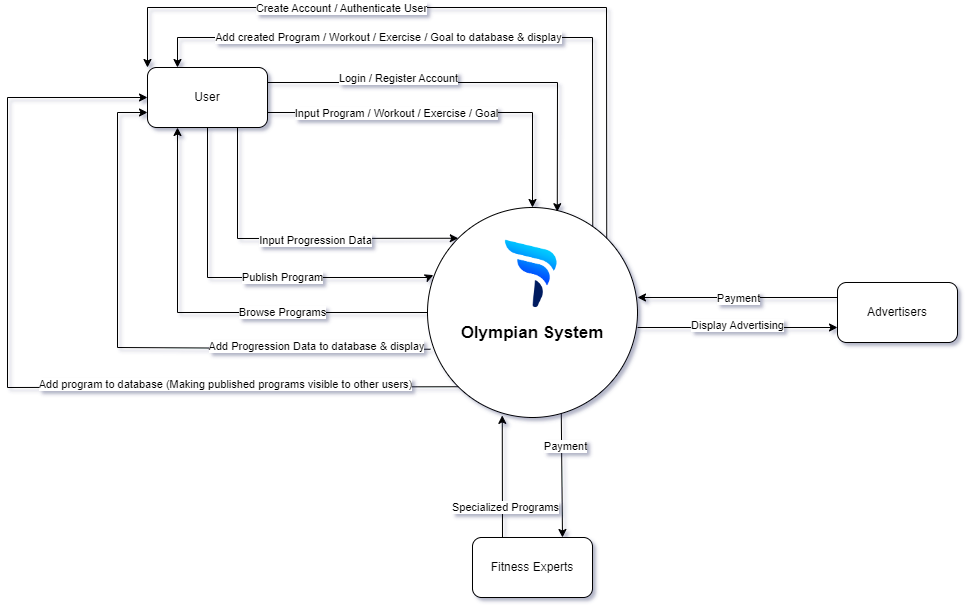
\includegraphics[scale=0.55]{system_context}
		\caption{System Context Diagram}
	\end{figure}

	\section{Project Overview}
	
	\subsection{Normal Behaviour}
	
	Normal behaviour for the application can be defined as the state of the available program when all FRs and NFRs are fulfilled. If an FR or NFR is not fulfilled, this is abnormal behaviour, and indicative of the occurrence of an undesired event.
	
	\subsection{Undesired Event Handling}
	
	\wss{How you will approach undesired events}
	
	An `undesired event' can comprise anything from incorrect user input to database failure to connectivity issues. 
	
	\textbf{Invalid User Input}: Whenever a user provides incorrect information to a form (e.g. an invalid email address during sign-up), an informative error message is displayed beneath the incorrectly filled field, and a visual queue is given in the form of highlighting the field in red to indicate error. To prevent annoying the user with error messages before they have actually made an error, forms will only display error messages after the first submit attempt. After an initial submit attempt, the error message will remain until the contents of the field are valid. This is to give the user information as to whether or not their entry is valid before having to submit again.
	
	\textbf{Connection/Database Failure}: If the application is unable to connect to the internet, and subsequently the server and database, an informative error message is displayed, informing the user to verify their internet connection. Note that a stretch goal for the future is to have the Olympian application save certain information locally to enable the user to perform certain functions offline. Changed local information would be synced with the database once connection is re-established. However, this is a stretch goal, and current requirements and designs list the database as the only information store, no data (other than an authentication token) is stored locally. If the database/server itself is failing, an appropriate message is displayed to the user. The message will indicate that the failure is not the fault of the user, but rather an internal failure outside of their control.
	\\
	
	Error messages are kept consistent and concise in format, to make errors easy for the user to recognize and act upon.
	
	
	
	
	
	\subsection{Component Diagram}
	
	\subsection{Connection Between Requirements and Design} \label{SecConnection}
	
	\wss{The intention of this section is to document decisions that are made
		``between'' the requirements and the design.  To satisfy some requirements,
		design decisions need to be made.  Rather than make these decisions implicit,
		they are explicitly recorded here.  For instance, if a program has security
		requirements, a specific design decision may be made to satisfy those
		requirements with a password.}
	
	\section{System Variables}
	
	\wss{Include this section for Mechatronics projects}
	N/A
	
%	\subsection{Monitored Variables}
	
%	\subsection{Controlled Variables}
	
%	\subsection{Constants Variables}
	
	\section{User Interfaces}
	
	\wss{Design of user interface for software and hardware.  Attach an appendix if
		needed. Drawings, Sketches, Figma}
	
	\section{Design of Hardware}
	
	\wss{Most relevant for mechatronics projects}
	\wss{Show what will be acquired}
	\wss{Show what will be built, with detail on fabrication and materials}
	\wss{Include appendices as appropriate, possibly with sketches, drawings, CAD, etc}
	
	Olypmian will run on mobile devices (e.g. iPhone, Samsung Galaxy) not designed or manufactured by the team.
	
	\section{Design of Electrical Components}
	
	\wss{Most relevant for mechatronics projects}
	\wss{Show what will be acquired}
	\wss{Show what will be built, with detail on fabrication and materials}
	\wss{Include appendices as appropriate, possibly with sketches, drawings,
		circuit diagrams, etc}
	
	N/A - See Section 9.
	
	\section{Design of Communication Protocols}
	
	\wss{If appropriate}
	
	\section{Timeline}
	
	\wss{Schedule of tasks and who is responsible}
	
	% \bibliographystyle {plainnat}
	% \bibliography{../../../refs/References}
	
	\newpage{}
	
	\appendix
	
	\section{Interface}
	
	\wss{Include additional information related to the appearance of, and
		interaction with, the user interface}
	
	\section{Mechanical Hardware}
	N/A
	
	\section{Electrical Components}
	N/A
	
	\section{Communication Protocols}
	The project employs Hyper Text Transfer Protocol (HTTP), enabling the client to communicate with the server and database through HTTP requests.
	
	\section{Reflection}
	
	The information in this section will be used to evaluate the team members on the
	graduate attribute of Problem Analysis and Design.  Please answer the following questions:
	
	\begin{enumerate}
		\item What are the limitations of your solution?  Put another way, given
		unlimited resources, what could you do to make the project better? (LO\_ProbSolutions)
		\item Give a brief overview of other design solutions you considered.  What
		are the benefits and tradeoffs of those other designs compared with the chosen
		design?  From all the potential options, why did you select documented design?
		(LO\_Explores)
	\end{enumerate}
	
\end{document}
